\documentclass{scrreprt}
\usepackage{graphicx}
\usepackage{float}
\usepackage{amsmath}

\title{Learning AFG \& DSO using Lissajous Figures}
\author{Jnanesh Sathisha Karmar \& Vivek Kumar}
\date{January 2026}

\begin{document}

\maketitle

\section{Explain the basic functions of an Arbitrary
Function Generator (AFG). What parameters can be controlled?}

An arbitrary function generator can be used to generate any form of input signal. It can be used to control the wave shape. Different wave shapes come included such as square, ramp, sine, pulse and noise, and many other wave shapes. There is also an option to choose an arbitrary waveform, where we can geberate any waveform of our choice.

\begin{figure}[h!]
        \centering
        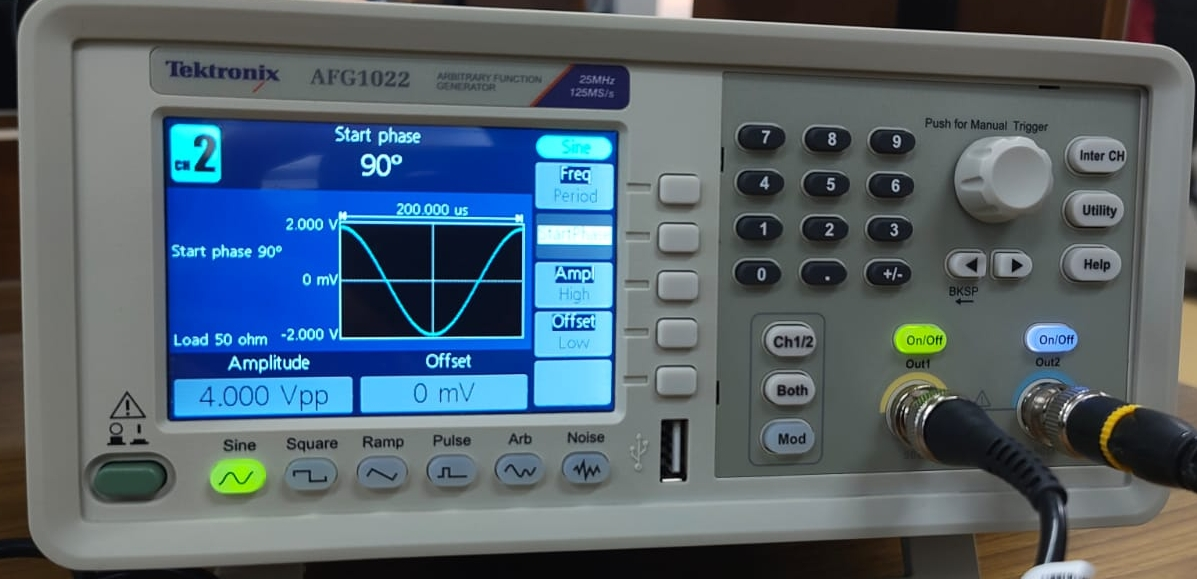
\includegraphics[width=0.8\linewidth]{figs/afg.jpeg}  
        \label{fig:afg}
\end{figure}

For each wave we can adjust the wave parameters like frequency, intital phase, amplitude, offset.

\begin{itemize}
        \item \textbf{Frequency}: It is the number of wave cycles that passes a fixed point per second.Along with frequency, there is an option to change the time period (inverse of frequency).       
        \item \textbf{Initial Phase}: We can adjust the initial phase of the signal. This is useful for creating a phase difference between 2 signals.
        \item \textbf{Amplitude}: We can also adjust the amplitude of the waveform in terms of Vpp(Voltage peak-peak). In the model available in the lab, the maximum amplitude is 10 Vpp.
        \item \textbf{Offset}: We can also shift the waveform vertically using this option. 
\end{itemize}

The model available in lab can produce atmost 2 signals, where each one of them can be independently controlled. There is also a numpad and a dial to manually adjust each parameter. 

\section{TODO! What are V/div and Time/div in a Digital
Storage Oscilloscope (DSO)? Why are they important?}

\begin{figure}[h!]
        \centering
        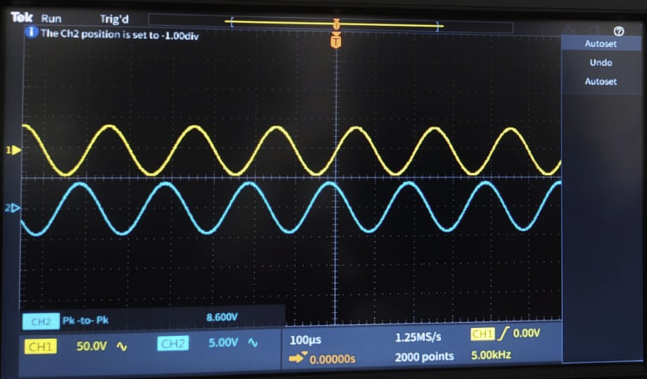
\includegraphics[width=0.8\linewidth]{figs/vdiv.png}  
        \label{fig:vdiv}
\end{figure}

They represent the scales of the time-domain graph used to visualize the waveform. V/div referes to Voltage/division, which is the y-axis scale. It helps us analyze the amplitude of the waveform. Time/div is the x-axis scale using which, we can infer the frequency of the waveform.

\section{Define phase difference between two
sinusoidal signals. How can it be measured using time-domain analysis?}
Phase difference between the two sinusoidal signals can be defined as the difference in the initial phase angle of the two waves (on a circle).

\begin{figure}[H]
        \centering
        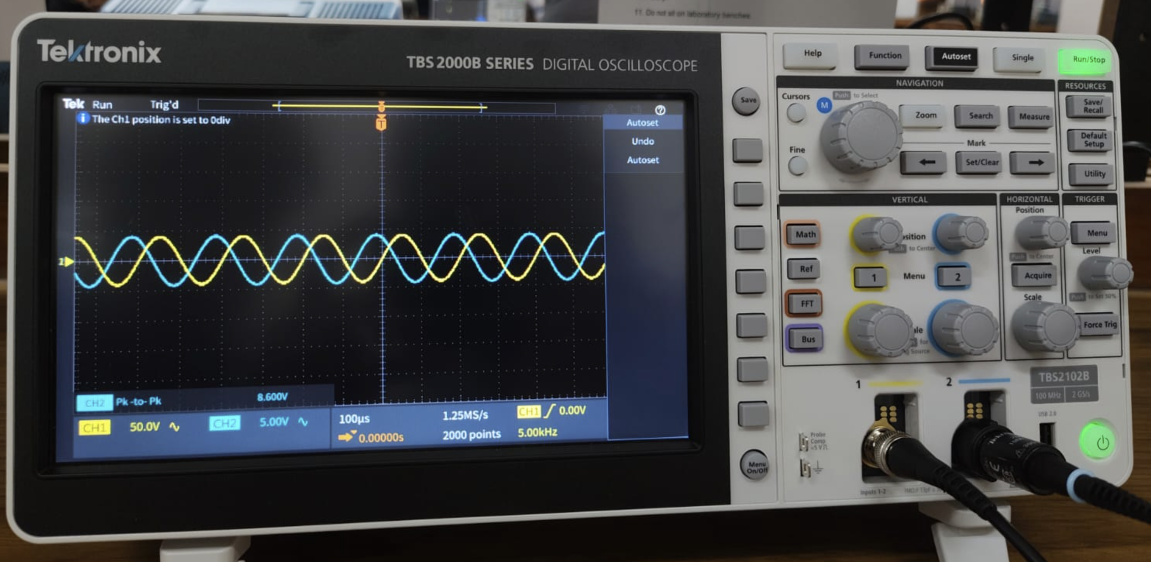
\includegraphics[width=0.8\linewidth]{figs/phasedso.png}  
        \label{fig:phasedso}
\end{figure}

We can find the phase difference of two signals with the same frequency by finding the peak-to-peak displacement in terms of phase. In the image above, the time period is 10 Time/div, and the time between two closest peaks is around 3.33 Time/div.\\ Hence in this case, $\Delta\phi = \frac{3.33}{10}\times2\pi = \frac{2\pi}{3}$
We can verify the above result by looking at the AFG used to generate these signals.

\begin{figure}[H]
        \centering
        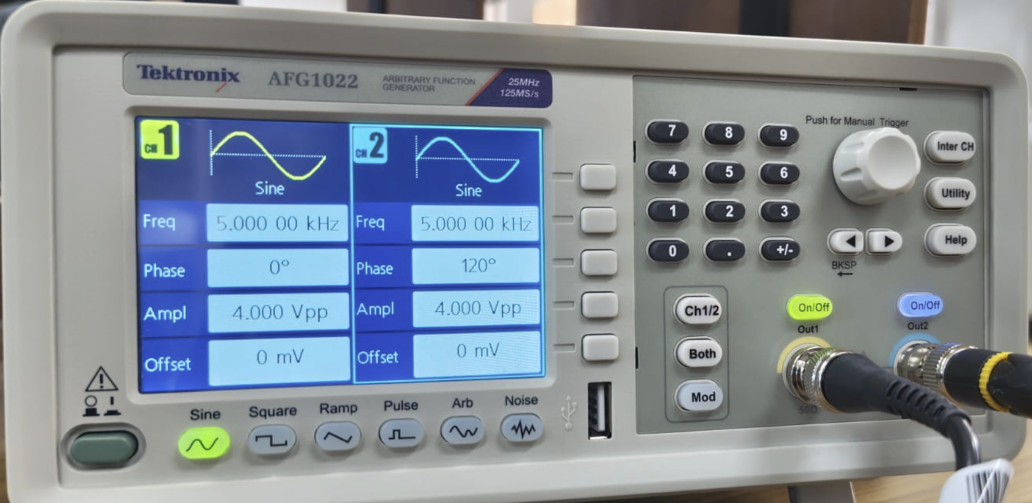
\includegraphics[width=0.8\linewidth]{figs/phaseafg.png}  
        \label{fig:phaseafg}
\end{figure}

\section{What is XY mode in a DSO? How is it
different from time-domain mode?}

XY mode is a useful tool which can be used to compare both the signals. Instead of the time-domain mode which shows the two waveforms as the function of time, the XY mode has one signal as a function of another. 

\begin{figure}[H]
        \centering
        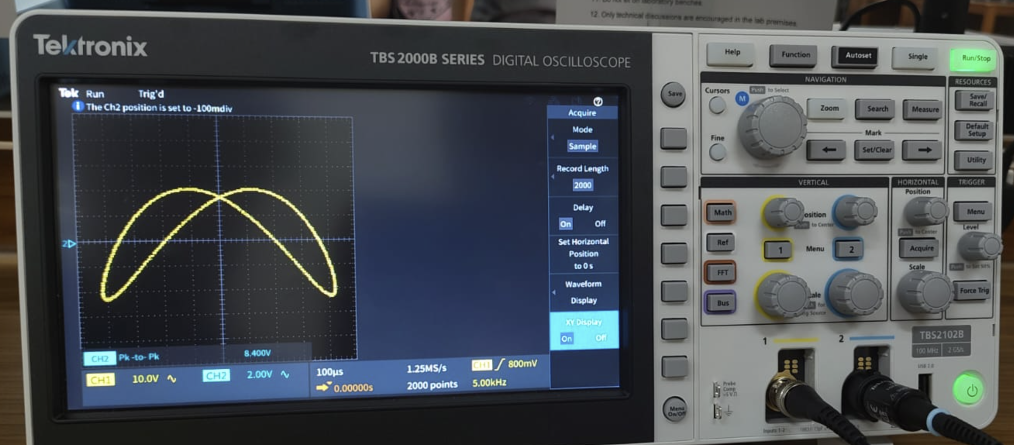
\includegraphics[width=0.8\linewidth]{figs/xymode.png}  
        \label{fig:xymode}
\end{figure}

The resulting shapes in the XY mode are called lissajous figures. Which can be useful to measure phase-difference and compare frequencies of two signals. 
The time-domain mode can also be viewed as applying a sawtooth waveform in the X direction. 

\section{TODO! - Draw and explain Lissajous figures for
(a) $0^\circ$ phase difference and (b) $90^\circ$ phase difference}

The lissajous figures for $0^\circ$ phase difference is a bounded straight line, as we can see in the figure above. The slope is the ratio of the amplitudes.
\begin{align}
        m = \frac{A_1}{A_2}
\end{align}

The lissajous figures for $90^\circ$ phase difference is a circle/ellipse with axes along coordinate axes, as we can see in the figure above. The eccentricity of the ellipse depends on the ratio of the amplitudes.
\begin{align}
        e = \sqrt{1-(\frac{A_1}{A_2})^2}
\end{align}


\end{document}

